\documentclass[varwidth=true]{standalone}
\usepackage{tikz}
\begin{document}
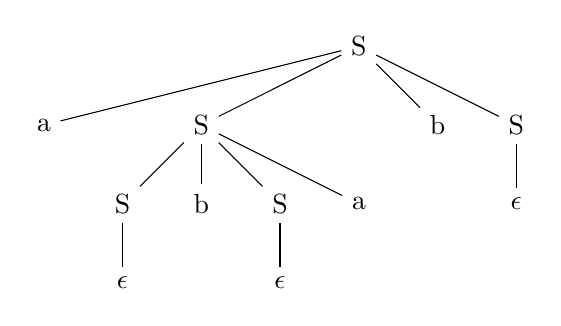
\begin{tikzpicture}
    \node (S0) at (0, 0) {S};

    \node (a0) at (-4, -1) {a};
    \draw (S0) -- (a0);
    \node (S1) at (-2, -1) {S};
    \draw (S0) -- (S1);
    \node (b0) at (1, -1) {b};
    \draw (S0) -- (b0);
    \node (S2) at (2, -1) {S};
    \draw (S0) -- (S2);

    \node (S10) at (-3, -2) {S};
    \draw (S1) -- (S10);
    \node (b1) at (-2, -2) {b};
    \draw (S1) -- (b1);
    \node (S11) at (-1, -2) {S};
    \draw (S1) -- (S11);
    \node (a1) at (0, -2) {a};
    \draw (S1) -- (a1);

     \node (e0) at (2, -2) {$\epsilon$};
     \draw (S2) -- (e0);

     \node (e1) at (-3, -3) {$\epsilon$};
     \draw (S10) -- (e1);
     \node (e2) at (-1, -3) {$\epsilon$};
     \draw (S11) -- (e2);
\end{tikzpicture}
\newline
\newline
\begin{tikzpicture}
    \node (S0) at (0, 0) {S};

    \node (a0) at (-2, -1) {a};
    \draw (S0) -- (a0);
    \node (S1) at (-1, -1) {S};
    \draw (S0) -- (S1);
    \node (b0) at (0, -1) {b};
    \draw (S0) -- (b0);
    \node (S2) at (2, -1) {S};
    \draw (S0) -- (S2);

    \node (a1) at (1, -2) {a};
    \draw (S2) -- (a1);
    \node (S10) at (2, -2) {S};
    \draw (S2) -- (S10);
    \node (b1) at (3, -2) {b};
    \draw (S2) -- (b1);
    \node (S11) at (4, -2) {S};
    \draw (S2) -- (S11);

     \node (e0) at (-1, -2) {$\epsilon$};
     \draw (S1) -- (e0);

     \node (e1) at (2, -3) {$\epsilon$};
     \draw (S10) -- (e1);
     \node (e2) at (4, -3) {$\epsilon$};
     \draw (S11) -- (e2);
\end{tikzpicture}
\end{document}